\documentclass[pdf,bookmarks,colorlinks=true]{IEEEtran}
\usepackage{times}
\usepackage{amsmath}
\usepackage{hyperref}
\usepackage{url}
\usepackage{psfrag}    %Shouldn't use this if you plan on using pdflatex!
\usepackage{graphicx}
\usepackage{wrapfig}   %for wrapping text around figures and tables

%Included for Gather Purpose in WinEdt only:
%input "rc.bib"

\title{\bf Survey Paper - Identifying Known Vulnerabilies in OSS libraries}

\author{Ronaldo Canesqui\\
Southern Adventist University\\
ronaldocanesqui@southern.edu
}
\graphicspath{{Images/}}
\begin{document}

\maketitle

\begin{abstract}

The use of open-source software libraries is experiencing exponential growth in the last decade. Modern software development practices fully embrace this model. Unfortunately, the advantages brought by reuse also brings the risk of vulnerabilities. The number of vulnerabilities found in open-source libraries is increasing faster than the number of available packages. How to leverage the power of open-source libraries and still manage the risk of vulnerabilities they carry is a problem that either remain ignored by many software engineers or present considerable challenges to them. Studies on dependencies management practices found that security criterion is not considered by the majority of developers and one-third of them are not aware of libraries update. This paper compiles the most recent studies on identifying known vulnerabilities on dependencies are presented, along with analytical data about vulnerability lifespan and current dependencies management practices.

\end{abstract}

%   \tableofcontents
%   \newpage

% \doublespace

\section{Introduction}
\label{sec:Introduction}

%\begin{itemize}
%\item
The use of open-source libraries is a reality in the software industry. In 2018, Synopsys\footnote{https://www.blackducksoftware.com/} found open-source code in more than 96\% of its audits\cite{Synopsys2019}. Open-source software (OSS) usage has increased exponentially during the last decade. The most popular source for libraries in the Java ecosystem, Maven Central Repository, growth 542.17\% from 2010 to 2016 \cite{Kula2018}. Another popular open-source repository for the Javascript ecosystem, npm growth from 0 packages at its creation in 2010 to 1,000,000 packages in 2019\footnote{https://snyk.io/blog/npm-passes-the-1-millionth-package-milestone-what-can-we-learn/ accessed 10/10/2019}.   
The figure~\ref{PackageEvolution} extracted from \cite{Decan} shows the number of packages evolution on other popular ecosystems.
\begin{figure}[h]
	\centering
	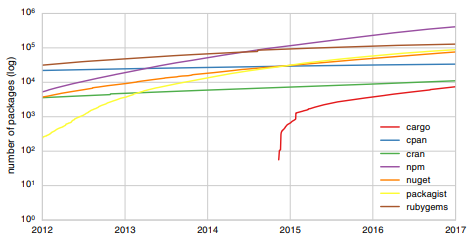
\includegraphics[scale=0.70]{PackagesEvolution.png}
	\caption{Evolution of the number of packages.}
	\label{PackageEvolution}
\end{figure}
%\item
How to leverage the power of open-source libraries and still manage the risk of vulnerabilities they carry is a problem that either remain ignored by many software engineers or present considerable challenges to them.

%\end{itemize}


A 2014 study from Sonatype determined that over 6\% of the download requests from the Maven Central Repository were for component versions that included known vulnerabilities. In their review of over 1,500 applications, each of them had an average of 24 severe or critical flaws inherited from their components \footnote{Report published January 02, 2015 at http://goo.gl/i8J1Zq.}.
A white paper produced by Contrast Security stated that over 25\% of all libraries downloaded from Maven Central Repository has a vulnerability. Only one vulnerable version of the Java GWT package was downloaded 17,666,703 times \cite{williams2012unfortunate}.
Among the 10 most popular npm packages, 6 present 1 or more vulnerabilities \footnote{https://snyk.io/blog/npm-passes-the-1-millionth-package-milestone-what-can-we-learn/ accessed 10/10/2019}.

In a study on security vulnerabilities impact \cite{Decan2018} the researchers found that out of 610,097 available packages (2017 data) 133,602 packages directly depend on a vulnerable package and 72,470 packages had at least one release that relies on a vulnerable package.
In the same study, they also found a crescent number or vulnerabilities in the npm repository. Figure~\ref{SVEvolution} shows the evolution of the number of vulnerabilities and the impact on dependent packages. Comparing 2014 and 2017 data, there is a clear increase on the impact that a vulnerable package (dotted lines) has over dependent packages (straight lines).

\begin{figure}[h]
	\centering
	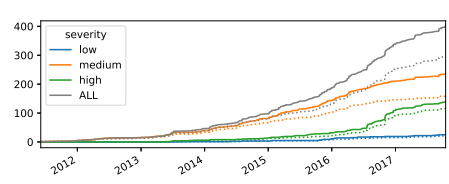
\includegraphics[scale=0.70]{SVEvolution.png}
	\caption{Evolution of the number of discovered vulnerabilities (straight lines) and corresponding distinct packages (doted lines) per severity.}
	\label{SVEvolution}
\end{figure}

%\end{itemize}

%\begin{itemize}
%\item
During this paper, the most recent studies on identifying known vulnerabilities on dependencies are presented, along with analytical data about vulnerability lifespan and current dependencies management practices.
%\item
The rest of this paper will cover studies on the vulnerability lifespan \ref{sec:VulnerabilityTimeFrame}, current dependencies management practices \ref{sec:DependenciesManagement}, proposed solutions on how to identify known vulnerabilities and evaluate updatability \ref{sec:IdentifyingknownVulnerabilities}, overview of the main challenges in the area \ref{sec:MainChallenges} and conclusion \ref{sec:Conclusion}.  

\section{Vulnerability Lifespan}
\label{sec:VulnerabilityTimeFrame}


%\begin{itemize}
%\item
To analyze the vulnerability lifespan the study \cite{Decan2018} used a 700 security vulnerabilities report made available by Snyk.io \footnote{https://snyk.io} and retrieved the list of corresponding releases from the open-source discovery service libraries.io \cite{Nesbitt2017}. Based on the list of releases, the researchers identified which ones were affected by the vulnerability.
Based on the relationship between package, vulnerability, first release data, and vulnerability discovery date, it was possible to trace a vulnerability timeframe.

\textbf{How long does the package remain vulnerable}
%\item
Figure~\ref{RemainsVulnerable} shows Kaplan-Meier estimator  curve \cite{Kaplan1958} for the event “vulnerability is fixed”. The data presented considers the date of the affected release and the date that the fix was available. After 10 months, there is a probability higher than 80\% that a high severity vulnerability is still not fixed.

\begin{figure}[h]
	\centering
	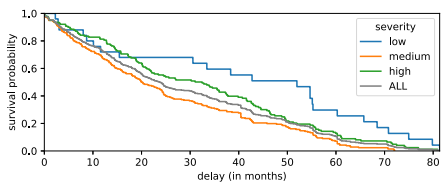
\includegraphics[scale=0.70]{RemainsVulnerable.png}
	\caption{Survival probability for event “vulnerability is fixed” w.r.t. the date of first affected release.}
	\label{RemainsVulnerable}
\end{figure}

%\end{itemize}


\textbf{When a vulnerability is discovered}
%\item 
Figure~\ref{WhenDiscovered} shows that most severities are discovered in old packages. 75\% of all vulnerabilities are found in libraries older than 13 months. Even not highlighted in the original study, the shorter wave in high severity vulnerabilities may suggest the higher priority in which they are handled, especially when compared to the low severity graph that shows smother curves. Most severities are found in packages older than 28 months.

\begin{figure}[h]
	\centering
	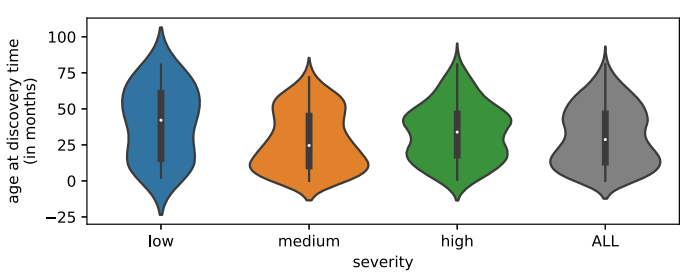
\includegraphics[scale=0.45]{WhenDiscovered.png}
	\caption{Violin plots of packages age at discovery time by vulnerability severity.}
	\label{WhenDiscovered}
\end{figure}

%\end{itemize}

\textbf{When a vulnerability is fixed}
%\item 
Most of the vulnerabilities are fixed between the discovery date and the public announcement. Figure~\ref{WhenIsFixed} shows that there is a probability of 50\% of a fix becomes available in the first month after discovery. And 80\% of all vulnerabilities are fixed between 12 and 13 months. After 20 months of the discovery all high severity vulnerabilities were fixed. Some medium severity vulnerabilities, according to the graph, will take more than 40 months to be fixed.

\begin{figure}[h]
	\centering
	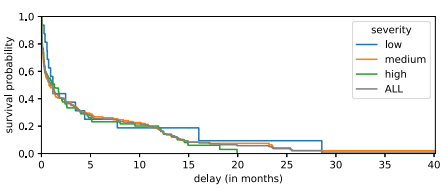
\includegraphics[scale=0.75]{WhenIsFixed.png}
	\caption{Survival probability for event "vulnerability is fixes" w.r.t. vulnerability discovery time.}
	\label{WhenIsFixed}
\end{figure}

%\end{itemize}


\textbf{When a vulnerability is fixed in a dependent package}
%\item 
The analysis of the impact on dependent packages is important due to the fast increase of dependencies. Figure~\ref{DependenciesGrowing} shows a more step curve when compared to the number of available packages (figure~\ref{PackageEvolution}). 
Figure~\ref{WhenIsFixedDependentPackages} shows that after 20 months, 100\% of high severity vulnerabilities are fixed while there are 40\% of the dependencies vulnerable at the same time. The slowness on updating dependencies found in this study is supported by similar findings in different studies covering a wide range of ecosystems such as SmallTalk\cite{Robbes:2012:DRA:2393596.2393662}, Pharo\cite{7332471}, Java \cite{7816485}, Apache products\cite{Bavota2015}, Windows ecosystem \cite{7163055}, and Javascript ecosystem \cite{Lauinger}.

\begin{figure}[h]
	\centering
	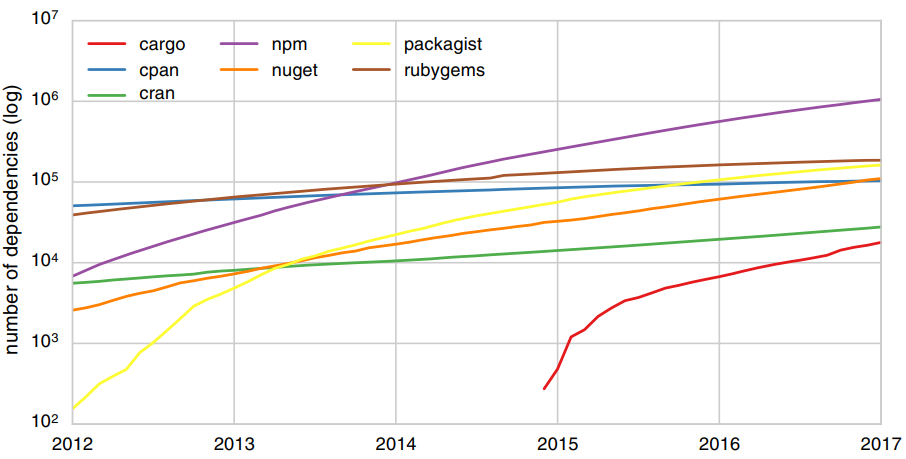
\includegraphics[scale=0.40]{DependenciesGrowing.png}
	\caption{Evolution of the number of dependencies (considering for each point in time the latest available
		release of each package).}
	\label{DependenciesGrowing}
\end{figure}

\begin{figure}[h]
	\centering
	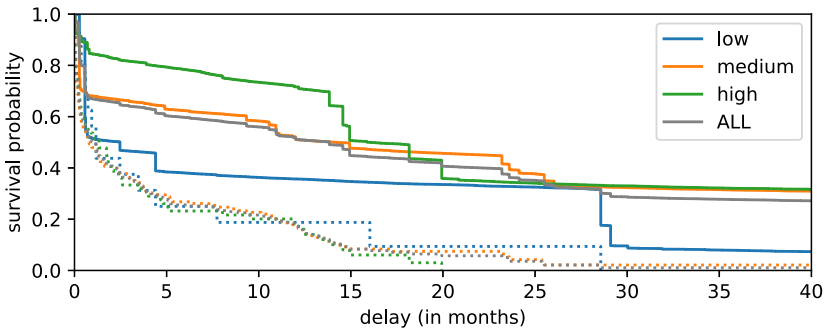
\includegraphics[scale=0.40]{WhenIsFixedDependentPackages.png}
	\caption{Survival probability for event “package is fixed” w.r.t. vulnerability discovery time. Dependent packages are
		shown as straight lines and upstream packages as dotted lines.}
	\label{WhenIsFixedDependentPackages}
\end{figure}

%\end{itemize}

\section{Current Dependencies Management Practices}
\label{sec:DependenciesManagement}


%\begin{itemize}
%\item
To understand the vulnerabilities lifespan it is required to understand current dependencies management practices specially on updating and selecting dependencies. A study \cite{Derr2017} conducted with 203 app developers from Google Play clarified the following research questions: {\em How frequently do developers update their apps/libs and what is their main motivation for updates?}
{\em What are possible reasons to not update dependencies and what solutions could app developers think of?}
%\item 
Based on the application maintainers' answers, the study concludes that 78\% of them do not have a fixed schedule for app updates (Figure~\ref{IsYourAppUpdatedFixedSchedule}) and only 33\% of them mention a library update as a reason to update their app (Figure~\ref{ForWhichReasonUpdate}). When the maintainers were questioned why do you update your app's libraries, 96.47\% of them answered bug fixing and 57.65\% mentioned security (figure~\ref{WhyDoYouUpdateYourLibrary}). Regarding library selection criteria, only 26.58\% answered security, even thought the answer update frequency is related and received 35.16\% of the votes (figure~\ref{LibrarySelectionCriteria}). When asked reasons why your app would include outdated libraries?, 57.03\% answered that the library was still working, 50\% answered to prevent incompatibilities and 32.81\% were unaware of updates (figure~\ref{ReasonsOutdatedLibrary}).

\begin{figure}[h]
	\centering
	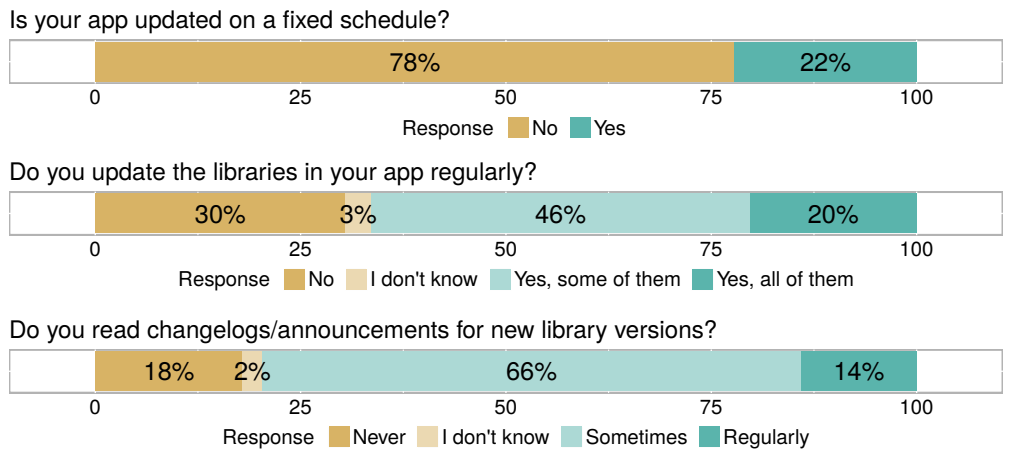
\includegraphics[scale=0.30]{IsYourAppUpdatedFixedSchedule.png}
	\caption{Anwsers for questions regarding app/library release frequency.}
	\label{IsYourAppUpdatedFixedSchedule}
\end{figure}
\begin{figure}[h]
	\centering
	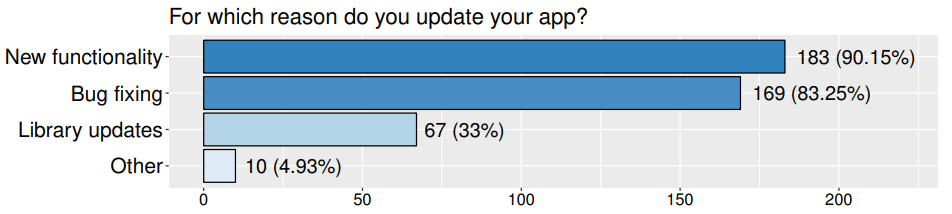
\includegraphics[scale=0.35]{ForWhichReasonUpdate.png}
	\caption{Answers for questions:For which reason do you update your app?}
	\label{ForWhichReasonUpdate}
\end{figure}
\begin{figure}[h]
	\centering
	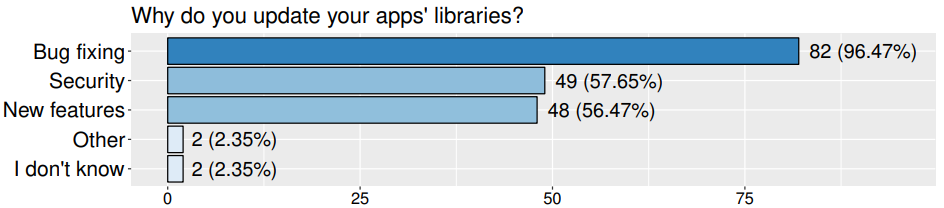
\includegraphics[scale=0.35]{WhyDoYouUpdateYourLibrary.png}
	\caption{Answers for questions: Why do you update your apps' libraries?}
	\label{WhyDoYouUpdateYourLibrary}
\end{figure}
\begin{figure}[h]
	\centering
	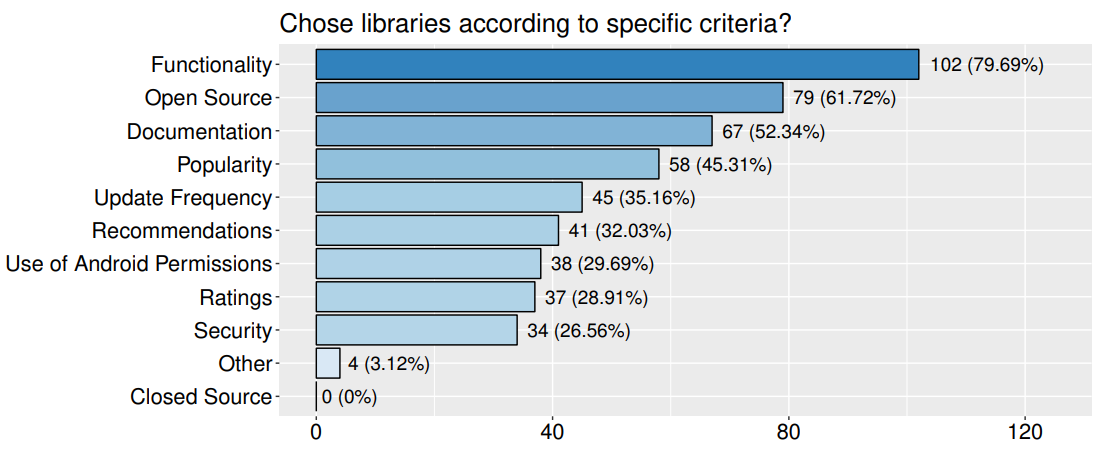
\includegraphics[scale=0.30]{LibrarySelectionCriteria.png}
	\caption{Answers for questions: Chose libraries according to specific criteria?}
	\label{LibrarySelectionCriteria}
\end{figure}
\begin{figure}[h]
	\centering
	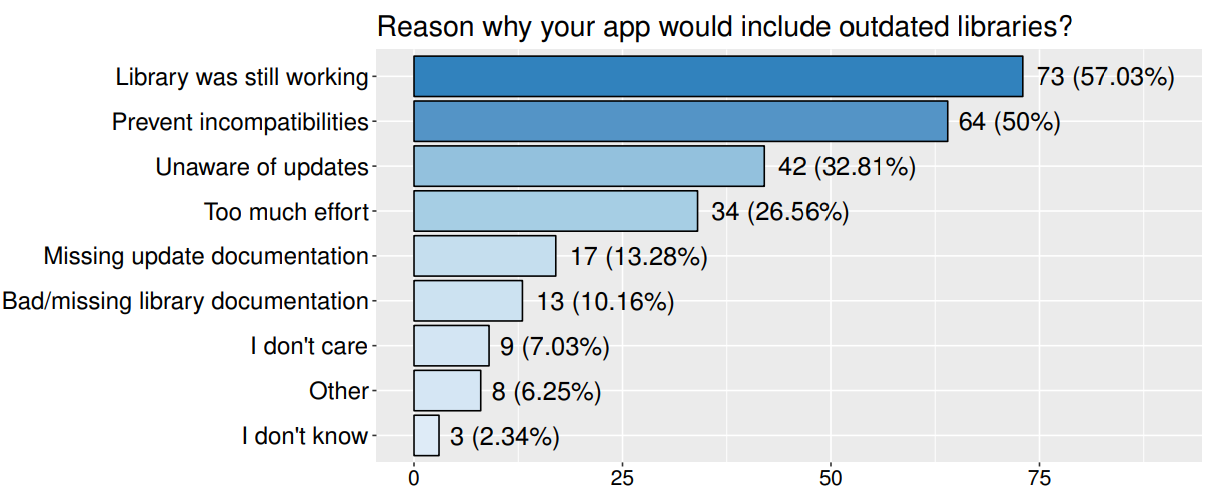
\includegraphics[scale=0.28]{ReasonsOutdatedLibrary.png}
	\caption{Answers for questions: Reason why your app would include outdated libraries?}
	\label{ReasonsOutdatedLibrary}
\end{figure}

%\begin{itemize}
%\item 
The study concludes that the main reasons to keep a library outdated are incompatibility prevention, unaware of updates and too much effort. Another study on this field \cite{Kula2018} reaches the same conclusion regarding why maintainers keep outdated dependencies. In the following sections, studies that proposed ways to deal with these  problems are presented along with their conclusions.

%\end{itemize}
\section{Identifying known Vulnerabilities and analyzing updatability}
\label{sec:IdentifyingknownVulnerabilities}

%\begin{itemize}
%\item
Various researchers have worked to solve the problem of know vulnerabilities in open-source packages and their dependencies. In this section, the most recent works will be presented along with their conclusions. This is not a comprehensive list but it offers a similar variety of methods and complexity of other works not covered here.

\textbf{Predicting vulnerabilities:}
%\begin{itemize}
%\item
Although the focus of this work is on papers that detect vulnerabilities using know vulnerabilities databases, it is worth mentioning that there is a branch of proposed solutions that operates identifying vulnerabilities based on a set of characteristics. Part of these solutions uses machine learning to identify vulnerabilities. One of these works \cite{Perl2015} mapped the CVE\footnote{Common Vulnerabilites and Exposures - https://cve.mitre.org/} entries to the commit that generated the vulnerability and trained an SVM-based \footnote{Support Vector Machine} model using the commit's metadata. According to the authors, this method reduced the number of false positives by 99\% when compared to Flawfinder\footnote{https://https://dwheeler.com/flawfinder/}. It was capable of detecting 53 of the 219 known vulnerabilities used in the study and only producing 36 false positives. The proposed solution analyses each commit and tries to predict the presence of vulnerabilities.
%\end{itemize}

\textbf{Measuring dependency freshness:}
%\begin{itemize}
%\item
The study \cite{Cox2015} proposes a method to measure the dependency freshness. The authors used information from the projects' {\em pom.xml} file to determine the libraries' version and used the Maven Central Repository to determine the release history for the library. Based on this information, the authors were able to classify each used component in a risk profile with 4 categories: low, moderate, high and very high.
To determine the relationship between their risk profile and the security vulnerabilities the researchers matched the dependencies list and tried to match with the CVE vulnerability database. They were able to find a correlation between their freshness index and the number of vulnerabilities. The median variance of the rating, the researchers were able to classify the systems according to dependency freshness:
\begin{itemize}
	\item \textbf{Stable} Systems with a stable dependency freshness rating. The system dependencies see little to no updates.
	\item \textbf{Improving} Systems with an increasing dependency freshness
	rating. Dependencies are updated faster than they are released.
	\item \textbf{Declining} Systems with a decreasing dependency freshness
	rating. Dependencies are updated slower than they are released.
\end{itemize}

The metrics presented have great potential in quantifying the dependency freshness. The method has at least one serious limitation: only direct dependencies can be measured, which can generate wrong classifications, especially when a direct dependency is updated but a transient dependency exists and is outdated.  

\textbf{Library updatability}
%\begin{itemize}
%\item
The study \cite{Cox2015} was able to correlated the library freshness with number of vulnerabilities. The finding that old libraries carry more vulnerabilities is also supported by other works \cite{Decan2018,Synopsys2019}. The study \cite{Derr2017} proposes an automated method to evaluate the updatability of dependencies. Their method consists of three steps: determine the API robustness, determine the library usage and determine the library updatability.
%\item
To determine the API robustness, the researchers extracted the public API from multiple versions of the same library, resulting in a library version/API pair list. According to the authors, this is a more fine-grained approach compared to \cite{Backes2016}. The authors then proceed with the library usage, where they inspect the bytecode looking for a call to the API. Finally, they matched the library version/API pair list with the library usage to produce the library updatability, which informs what is the latest version the API can be updated to without causing incompatibilities.

The authors test their approach analyzing 98 libraries and 1,246,118 apps from Google Play. The results show that in 85.6\% of the cases the identified library can be upgraded by at least one version (Upgrade1+) and on 48.2\% of the cases the library can be updated to the most current version simply by replacing the old library, without any code change. Figure~\ref{LibraryUpdatability} shows the libraries' updatability from their study.
 
\begin{figure}[h]
	\centering
	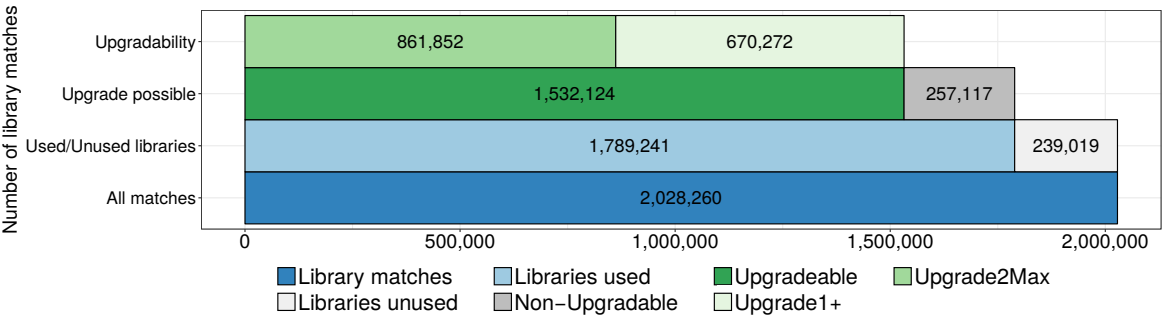
\includegraphics[scale=0.28]{LibraryUpdatability.png}
	\caption{Library updatability of current apps on Google Play.}
	\label{LibraryUpdatability}
\end{figure}


%\end{itemize}

\textbf{Vulnerability Alert Service (VAS)}
%\begin{itemize}
%\item
The Vulnerability Alert Service (VAS) is proposed by \cite{Cadariu2015}. Their focus is to increase the awareness about known vulnerabilities by making it part of the software quality process. The overall process is illustrated in figure ~\ref{VASProcess}. First, the target project has its dependencies extracted and recognized. Then, list of dependencies is analyzed by the matching task, which tries to match the dependency with an entry from the vulnerability disclosures, in this study a CVE entry. Upon a successful match, an alert is produced which is consumed by a human operator. The authors extended the OWASP Dependency Check Tool to extract the dependencies list from Maven {\em pom.xml} files and used this tool as the vulnerability checker described in the diagram.
%\item
The conclusion of this work shows a false positive rate of over 70\%, but the authors state that the rate is smaller when the solution was actually deployed. 
The researchers affirm that the high false-positive can be caused by situations like the MySQL-connector jar which is flagged with the vulnerabilities of the MySQL database server. The evaluation with the human operators shown that despite the false positive rate, an alert system was considered useful. Even the authors were satisfied with the operators' evaluation only direct dependencies can be identified by their method.

\begin{figure}[h]
	\centering
	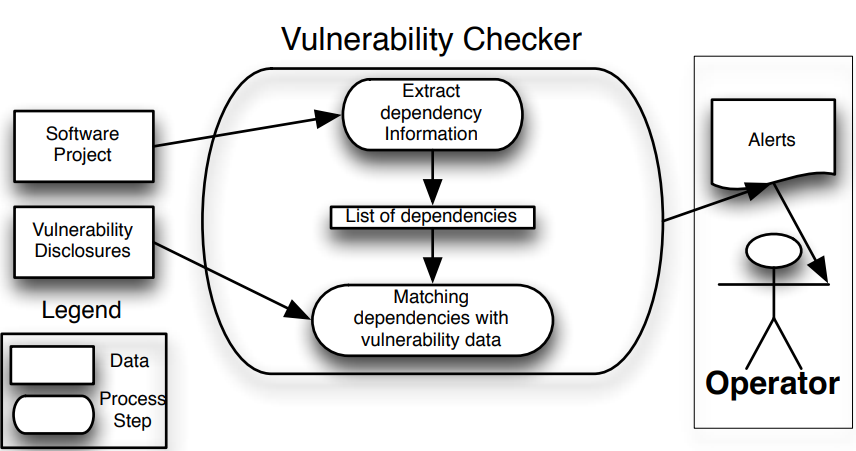
\includegraphics[scale=0.28]{VASProcess.png}
	\caption{The Vulnerability Alert Service process}
	\label{VASProcess}
\end{figure}
%\end{itemize}


\textbf{Code-based vulnerability identification}
%\begin{itemize}
%\item
The study \cite{Ponta2018} uses a method to identify vulnerabilities that, according to the authors, is more accurate than the methods proposed so far. Their work aims to answer the questions: {\em does my application is vulnerable if it uses a vulnerable dependency?} The researchers claim that this is not always the case and other studies failed to answer this question. The authors state that the software that contains a certain library that has known vulnerability does not need to be subject to costly efforts if proven that the vulnerability does not present harm. This way, the fix can be applied in the subsequent releases under no additional cost. Conceptually their solution can be used on any ecosystem, but their implementation is based on the Java ecosystem and the Maven Central Repository. They used the project’s {\em pom.xml} file to determine the dependencies. After the dependencies are determined, they remove all dependencies classified as provided and test, since those will not be deployed. Then the halted libraries\footnote{Libraries that do not receive an updated in a certain period of time define by the study.} are identified and removed. 
%\item
One key aspect for this approach to work is a database vulnerability that contains the meta-data about the library, such as name and version according to Maven Central Repository, the vulnerable source code and the source code for the fix. Using this database is possible to associate the dependency identified previously and the vulnerability, along with the source code involved in the vulnerability. This database was manually produced by the authors using CVE entries and it covers 90\% of Java ecosystem vulnerabilities.
%\item
The authors used static and dynamic analysis to determine if the vulnerable code is reachable. The dynamical analysis is done by instrumenting the vulnerable code and running automated and manual tests.
Their solution will notify the user if the vulnerability has impact on the application, meaning, the vulnerable code can be reached and also notify about the presence of halted libraries.

%\item
Other studies from the same authors use the same method to identify known vulnerabilities but focus on different aspects of the solution. \cite{Plate2015} introduces a simpler but very similar method to the one previously described. It was presented as a proof-of-concept and targets performance comparison between their approach, OWASP Dependency Check and two commercial tools.  \cite{pashchenko2018esem} focuses on how the impact of know vulnerabilities is inflated since other studies are counting vulnerable dependencies that are not deployed, such as libraries that are only used during tests. 
%\end{itemize}

%\item
According to the researchers, the code-based identification method is superior to the ones based on meta-data, since it does not suffer from problems such library artifacts renamed, named inconsistently and the fact that libraries can be extracted and repacked as a single self-contained archive. All these problems affect meta-data based identification. In the study \cite{Plate2015} the authors claim this method is the state-of-art in the filed.
This method is the officially recommended by SAP to scan projects and it is used by over 500 distinct development projects.

%\end{itemize}

\section{Main Challenges}
\label{sec:MainChallenges}


%\item
Although other studies on identifying known vulnerabilities do not explicitly mention the main challenges while trying to associate a library with a known vulnerability the study \cite{Plate2015} does. Their challenges can be observed implicitly on all studies compiled in this work. To establish this relationship, information from different sources needs to be integrated, such as vulnerabilities database, libraries repository, and source code repository.
The authors state that multiple problems hinder this integration, requiring ad-hoc and technology-specific solutions. Such problems hindered the detection of known vulnerabilities. As evidence, all studies compile in this work have at least one manual step that in its absence, the work would be infeasible.
\begin{itemize}
%\item
\item
{\em Non-uniform reporting of products affected by a vulnerability} - In some cases, only the CPE of the respective library is mentioned, in other cases, products or libraries using the library are also listed.  
%\item
\item
{\em Vulnerability and dependency management make use of different naming schemes and nomenclatures} - CPE does not straight map to packages repositories such as Maven or npm.
%\item
\item
{\em Vulnerabilities and VCS information of the respective patch are not linked in a systematic and machine-readable fashion} - While committing a fix to the repository, developers do not have a standard way to refer to the CPE.

\end{itemize}
%\item
Improved know vulnerabilities databases and standard ways to identify the OSS libraries in the repositories and commits would increase significantly the automation level and the impact of the available solutions.

\section{Conclusion}
\label{sec:Conclusion}

There are several works that tackle different aspects of the known vulnerability problem. Some of them directly identify the vulnerability, such as the code-based method, while others offer an indication of possible vulnerabilities such as the dependency freshness metrics. There is no one solution that will fit the majority of cases. Even in production-ready solutions, there is a dependency on technology-specific details, ad-hoc adjustments, and manually built databases. This paper covered a set of different solutions that can help software development practitioners to streamline their dependency management process.  

\bibliographystyle{IEEETrans}
\bibliography{./rc}


\end{document}
